\subsection{Spot the Straight Line on the Smith Chart!}

\begin{tcolorbox}[colback=gray!10, colframe=black, title=E9G07] What is the only straight line shown on the Smith chart? 

\begin{enumerate}[label=\Alph*.]
    \item The reactance axis
    \item The current axis
    \item The voltage axis
    \item \textbf{The resistance axis}
\end{enumerate} \end{tcolorbox}

\subsubsection{Understanding the Smith Chart}

The Smith chart is a graphical representation used in electrical engineering, particularly for impedance matching in radio frequency applications. It is a polar plot that allows for visualization of complex impedances and their relationships in transmission lines.

One important feature of the Smith chart is the representation of various axes. The chart consists of a series of circles and lines that help in visualizing the resistive and reactive components of impedances. In particular, certain axes can be represented either as straight lines or curves on the Smith chart.

\subsubsection{Analysis of Given Choices}

To analyze the options provided in the question:

\begin{itemize}
    \item \textbf{A: The reactance axis} - The reactance axis consists of curved lines that represent different values of reactance. Hence this is not the straight line.
    \item \textbf{B: The current axis} - There is no specific current axis defined in conventional Smith chart terminology. This option is also not a straight line.
    \item \textbf{C: The voltage axis} - Similar to the current axis, there is no designated voltage axis per Smith chart conventions.
    \item \textbf{D: The resistance axis} - The resistance axis is the only line that remains straight across the Smith chart. 
\end{itemize}

Thus, the correct choice is D: The resistance axis.

\subsubsection{Related Concepts}

In order to correctly interpret and utilize the Smith chart, one must have a basic understanding of the following concepts:

1. \textbf{Impedance:} Impedance is the total opposition to the flow of electric current in a circuit, comprising resistive and reactive components.
2. \textbf{Reactance:} Reactance refers to the imaginary part of impedance and can be capacitive or inductive.
3. \textbf{Reflection Coefficient:} This parameter indicates how much of an incident wave is reflected back due to impedance mismatches.

\subsubsection{Visual Representation}

A representation of the Smith chart can be sketched using the TikZ package in LaTeX. Below is a simple outline of a Smith chart that can be drawn:

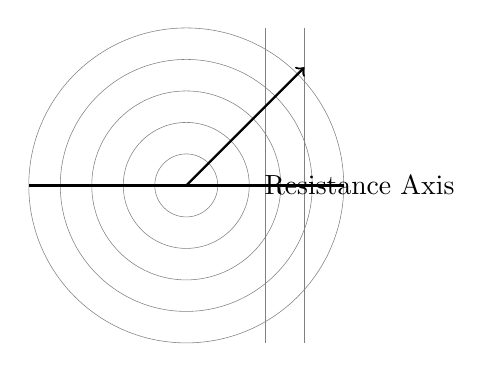
\begin{tikzpicture}
    \draw [very thin, gray] (0,0) circle(2cm);
    \foreach \r in {0.2,0.4,0.6,0.8}
        \draw [very thin, gray] (0,0) circle(\r*2cm);
    \foreach \x in {1.0,1.5}
        \draw [very thin, gray] (\x, -2) -- (\x,2);
    
    \draw[thick] (-2,0) -- (2,0); % Resistance axis
    \draw[thick,->] (0,0) -- (1.5,1.5); % Example line
    \node at (2.2,0) {Resistance Axis};
\end{tikzpicture}

This simple representation does not include all features of a complete Smith chart but indicates the important components discussed. 

In conclusion, understanding the structure and the primary functions of different components within a Smith chart is crucial for successfully engaging with RF circuits and analyzing their behavior.
